% PhD dissertation template for ECE Dept at UMassD
%
%

\documentclass[
12pt,
letterpaper,
% draft  % Uncomment to enable draft mode
]
{report}

\usepackage[noadjust]{cite}
\usepackage{hyperref}   % Generates bookmarks on pdf viewers
\usepackage{setspace}
\usepackage{amsmath}
\usepackage{amsfonts}
\usepackage{amssymb}
\usepackage[]{graphicx}
% \usepackage{fancyvrb}   % Fancy verbatim package 
% \usepackage{bm}   % Bold math symbols
\usepackage{stmaryrd}
\usepackage{subfig}
\usepackage{algorithm}
\usepackage{algpseudocode}
\usepackage{ragged2e}
\usepackage[]{appendix}
\numberwithin{equation}{chapter}

% --------------------------------------------
% Setup to get the chapter names to appear in 
% proper format in the table of contents
% 
\usepackage[titles, subfigure]{tocloft}
\usepackage{calc}
\renewcommand{\cftchappresnum}{Chapter }
\renewcommand{\cftchapaftersnum}{:}
\addtolength\cftchapnumwidth{\widthof{Chapter}}
% ---------------------------------------------

% Letterpaper size: 8.27in x 11in
% % Margin reset using Geometry package (easiest to use)
\usepackage[top=1in, bottom=1.3in,
left=1.5in, right=1.1in,
footskip=0.3in]{geometry}

% Specify the path containing your figures. This allows you to simply specify the figure filename with \includegraphics rather than explicitly specify the path to the figure file.
\graphicspath{{../figures/pdf/}}
\renewcommand{\figurename}{Fig.}

\newcommand{\thesistitle}{Awesome thesis title}
\newcommand{\authorname}{John Doe}

% -------------------------------------------
% Following snippet enables proper formatting of author names
% in the bibliography. This template uses IEEE bibliography format
% Ref: http://www.michaelshell.org/tex/ieeetran/bibtex/
%
% Define \bstctlcite
\makeatletter
\def\bstctlcite{\@ifnextchar[{\@bstctlcite}{\@bstctlcite[@auxout]}}
\def\@bstctlcite[#1]#2{\@bsphack
 \@for\@citeb:=#2\do{%
   \edef\@citeb{\expandafter\@firstofone\@citeb}%
   \if@filesw\immediate\write\csname#1\endcsname{\string\citation{\@citeb}}\fi}%
 \@esphack}
\makeatother
% -------------------------------------------

% ------------------------------------------
% \raggedright

\begin{document}
\bstctlcite{IEEEexample:BSTcontrol} % Control for IEEEtrans.bst to disable repeated name

% % -------------------Front Matter-----------------------
\setcounter{page}{1}
\pagenumbering{roman}  % Front matter needs to use roman page numbering

% Title page for PhD dissertation
% Saurav R. Tuladhar
% Oct 28, 2015

\thispagestyle{empty}
%\enlargethispage{0.8in} % default textheight is 592pt = 8.2inch
\newgeometry{margin=1.5in}
\doublespacing
\begin{center}

University of Massachusetts Dartmouth \\
College of Engineering \\


\vspace*{5em}
{\sc Awesome thesis title} \\

\vspace*{5em}
A Dissertation in 

Electrical Engineering 

by

\authorname

\vspace*{7em}
Submitted in Partial Fulfillment of the 

Requirements for the Degree of \\ Doctor of Philosophy 

\vfill
January 2016

\end{center}
\restoregeometry
%%% Local Variables:
%%% mode: latex
%%% TeX-master: "main"
%%% End:

\clearpage

%Permission to UMassD
\thispagestyle{empty} %No page number
\doublespacing
\begin{flushleft}
I grant the University of Massachusetts Dartmouth the non-exclusive right to use
the work for the purpose of making single copies of the work available to the public
on a not-for-profit basis if the University's circulating copy is lost or destroyed.

\vskip 2em
\hfill \rule{2.73in}{0.5pt} \\
\vspace*{-0.5em}
\hspace*{3.17in}\authorname\\
\vspace{1em}
\hfill Date \rule{2.35in}{0.5pt} 
\end{flushleft}

%%% Local Variables:
%%% mode: latex
%%% TeX-master: "main"
%%% End:

\clearpage

\setcounter{page}{2}
% Signature page 
% Comment: use uniform units for length
\enlargethispage{3cm}
\newenvironment{changemargin}[2]{%
  \begin{list}{}{%
       \setlength{\textwidth}{6in} % 8.5 - 1.5 - 1 
       \setlength{\voffset}{0.5in}  % One inch + whatever set here
       \setlength{\marginparsep}{0in}
       \setlength{\topmargin}{0in}%
       \setlength{\headheight}{0in}
       \setlength{\headsep}{0in}
       \setlength{\footskip}{0in}
       \setlength{\footnotesep}{0in}
       \setlength{\rightmargin}{#2}%
       \setlength{\leftmargin}{#1}%
    }%
  \item[]}{\end{list}}
\thispagestyle{empty}
\newcommand{\titlesep}{0.15in}
\singlespacing
\begin{changemargin}{0in}{0in}
  \begin{flushleft}
    \normalsize
    We approve the dissertation of \authorname \par
    \vskip 0.05in
    \hspace{4.45in} Date of Signature
    \vskip 0.1in
    \rule{0.55\textwidth}{0.5pt} \hfill \rule{1.4in}{0.5pt} \\
    John R. Buck \\ Professor, Department of Electrical and Computer Engineering \\ Dissertation Advisor

    \vskip \titlesep    
    \rule{0.55\textwidth}{0.5pt} \hfill \rule{1.4in}{0.5pt} \\ 
    Dayalan P. Kasilingam \\ Professor, Department of Electrical and Computer Engineering \\ Dissertation Committee 
    
    \vskip\titlesep
    \rule{0.55\textwidth}{0.5pt} \hfill \rule{1.4in}{0.5pt} \\
    Paul J. Gendron \\ Assistant Professor, Department of Electrical and Computer Engineering \\ Dissertation Committee

    \vskip\titlesep
    \rule{0.55\textwidth}{0.5pt} \hfill \rule{1.4in}{0.5pt} \\
    Christ D. Richmond \\ Senior Technical Staff, MIT Lincoln Laboratory    \\ Dissertation Committee 

    \vskip\titlesep
    \rule{0.55\textwidth}{0.5pt} \hfill \rule{1.4in}{0.5pt} \\
    Raj R. Nadakuditi \\ Assistant Professor, University of Michigan \\ Dissertation Committee 

    \vskip \titlesep
    \rule{0.55\textwidth}{0.5pt} \hfill \rule{1.4in}{0.5pt} \\
    Hong Liu \\ Graduate Program Director\\ Department of Electrical and Computer Engineering 
    
    \vskip \titlesep
    \rule{0.55\textwidth}{0.5pt} \hfill \rule{1.4in}{0.5pt} \\
    Antonio H. Costa \\ Chairperson, Department of Electrical and Computer Engineering  

    \vskip \titlesep
    \rule{0.55\textwidth}{0.5pt} \hfill \rule{1.4in}{0.5pt} \\
    Robert E. Peck \\ Dean, College of Engineering 

    \vskip \titlesep
    \rule{0.55\textwidth}{0.5pt} \hfill \rule{1.4in}{0.5pt} \\
   Tesfay Meressi\\
   Associate Provost for Graduate Studies

  \end{flushleft}

\end{changemargin}
\clearpage
%%% Local Variables:
%%% mode: latex
%%% TeX-master: "main"
%%% End:

\clearpage

\doublespacing
\chapter*{Abstract}
\thesistitle
\begin{flushleft}
by \authorname \\
\end{flushleft}

A long time ago in a galaxy far, far away....

%%% Local Variables:
%%% mode: latex
%%% TeX-master: "main"
%%% End:

\clearpage

\doublespacing
\chapter*{Acknowledgments}
Thank you guys!
%%% Local Variables:
%%% mode: latex
%%% TeX-master: "main"
%%% End:

\clearpage

% Table of contents
\renewcommand\cftchapfont{\normalfont}
\renewcommand\cftchappagefont{\normalfont}
\renewcommand{\contentsname}{Table of contents}
\setlength{\cftbeforechapskip}{0.05in}
\onehalfspacing
\setcounter{tocdepth}{2}
\tableofcontents
\clearpage 

% List of figures
\setlength{\cftfigindent}{0em}
\setlength{\cftbeforefigskip}{0.05in}
\renewcommand{\listfigurename}{List of figures}
\addcontentsline{toc}{chapter}{\listfigurename{}}
\listoffigures
\clearpage

% \addcontentsline{toc}{chapter}{List of Tables}
% \listoftables
% \newpage 

% --------- End of Front Matter---------------------------------

% ---------- Start of Chapters----------------------------------

%\onehalfspacing
\doublespacing
\thispagestyle{plain}
\setcounter{page}{1}  % Restart counter
\pagenumbering{arabic}

% Main body
% Macro for various math symbols
% You can define your own following the examples below
% Inherited from JRB and KEW

\newcommand{\Cov}{\boldsymbol{\Sigma}}
\newcommand{\cov}{\sigma}
\newcommand{\Covdmr}{\Cov_{\rm DMR}}
\newcommand{\eval}{\gamma}
\newcommand{\Eval}{\boldsymbol{\Gamma}}
\newcommand{\evec}{\boldsymbol{\xi}}
\newcommand{\Evec}{\boldsymbol{\Xi}}
\newcommand{\sampCov}{{\bf S}}
\newcommand{\sampcov}{s}
\newcommand{\sampCovdmr}{\sampCov_{\rm DMR}}
\newcommand{\sampeval}{g}
\newcommand{\sampEval}{{\bf G}}
\newcommand{\sampevec}{{\bf e}}
\newcommand{\sampEvec}{{\bf E}}
\newcommand{\herm}{^{\rm H}}
\newcommand{\trans}{^{\rm T}}
\newcommand{\rep}{{\bf v}}        % planewave replica
\newcommand{\repmat}{{\bf V}}     % replica matrix
\newcommand{\sigamp}{b}
\newcommand{\wmvdr}{{\bf w}_{\rm MVDR}}
\newcommand{\wdmr}{{\bf w}_{\rm DMR}}
\newcommand{\dl}{\delta}
\newcommand{\dlmin}{\dl_{min}}
\newcommand{\wconv}{{\bf w}_{\rm conv}}
\newcommand{\nulldepth}{\mbox{ND}}
\newcommand{\replook}{\rep_0}
\newcommand{\repint}{\rep_I}
\newcommand{\tsp}{^{\rm T}}
\newcommand{\inv}{^{-1}}
\newcommand{\limrmt}{\lim_{RMT}}
\newcommand{\eig}{\operatorname{eig}}
\newcommand{\diag}{\operatorname{diag}}
\newcommand{\sign}{{\operatorname{sgn}}}

% Formatting commands
\newcommand{\mbf}[1]{\mathbf{#1}}
\newcommand{\fig}{Fig.~}
\newcommand{\sect}{Sec.~}
\newcommand{\eqn}{Eq.~}
\newcommand{\nth}{^{\rm th}}
\newcommand{\norm}[1]{||#1||}

%%% Local Variables: 
%%% mode: latex
%%% TeX-master: "main"
%%% End:  % Macro definitions saved in  mycommands.tex

\chapter{Introduction}
\label{cha:introduction}

Introduction to this dissertation...

\begin{figure}[!ht]
  \centering
  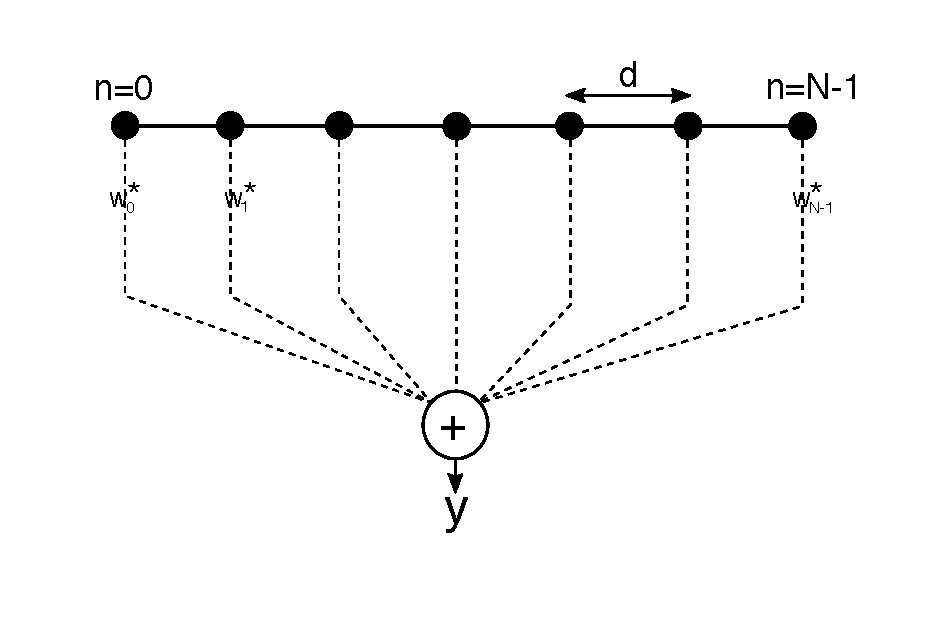
\includegraphics[width=3in]{beamforming.pdf}
  \caption{Beamforming}
\end{figure}

%%% Local Variables:
%%% mode: latex
%%% TeX-master: "main"
%%% End:


\chapter{Literature review}
\label{cha:literature-review}


%%% Local Variables:
%%% mode: latex
%%% TeX-master: "main"
%%% End:
 

\chapter{Conclusion}
\label{cha:conclusion}


%%% Local Variables:
%%% mode: latex
%%% TeX-master: "main"
%%% End:


% ---------- End of Chapters----------------------------------
% % Back matter
% \e{IEEEexample:BSTcontrol}

\begin{appendices}
\addtocontents{toc}{\def\protect\cftchappresnum{Appendix }}
\addtocontents{toc}{\addtolength\cftchapnumwidth{\widthof{ix }}}
\chapter{Proof of xyz}% on MVDR zeros}
\label{app:proof}

% =====================================================================
\chapter{Evaluation of derivatives}
\label{app:derivative}

%%% Local Variables:
%%% mode: latex
%%% TeX-master: "main"
%%% End:
   % Define appendix in appendix.tex file
\end{appendices}
\clearpage


% Un-comment the section below to enable bibliography
% All bibtex entries are stored in ../refs/myrefs.bib
% This requires IEEEtran.bst be present in ../refs/
%
% Bibliography
% \addcontentsline{toc}{chapter}{Bibliography}
% \bibliographystyle{../refs/IEEEtran}
% \bibliography{../refs/IEEEabrv,../refs/myrefs}

\end{document}

%%% Local Variables:
%%% mode: latex
%%% TeX-master: "main"
%%% End:

